\documentclass[aspectratio=169]{beamer}

\usepackage{natbib}
\usepackage{graphicx} % more modern
\graphicspath{{./diagrams/}}
\DeclareGraphicsExtensions{.pdf,.jpeg,.png}

% --------------- math notations ---------------
% This file defines notation to be used
\global\long\def\outputIndex{j}
\global\long\def\dataIndex{i}
\global\long\def\dataIndexTwo{j}
\global\long\def\latentIndex{j}

\global\long\def\inputSpace{\mathcal{X}}

\global\long\def\conditionalCovariance{\boldsymbol{\Sigma}}

\global\long\def\fantasyDim{r}
\global\long\def\dataDim{p}
\global\long\def\latentDim{q}
\global\long\def\inputDim{q}
\global\long\def\numLayers{\ell}
\global\long\def\numData{n}
\global\long\def\numTime{T}
\global\long\def\numTasks{m}
\global\long\def\numSequences{s}
\global\long\def\numInducing{m}
\global\long\def\numNeighbors{K}
\global\long\def\numHidden{h}
\global\long\def\numComponents{m}
\global\long\def\numBasisFunc{m}
\global\long\def\iterNum{k}
\global\long\def\maxIters{K}

\global\long\def\rbfWidth{\ell}
\global\long\def\lengthScale{\ell}
\global\long\def\binomProb{\pi}

\global\long\def\dataStd{\sigma}
\global\long\def\featureStd{\varsigma}

\global\long\def\heaviside{H}
\global\long\def\errorFunction{E}
\global\long\def\likelihoodFunction{L}
\global\long\def\likelihoodBound{\mathcal{L}}
\global\long\def\lagrangian{L}

\global\long\def\parameterScalar{\theta}
\global\long\def\parameterVector{\boldsymbol{\parameterScalar}}
\global\long\def\parameterMatrix{\boldsymbol{\Theta}}

\global\long\def\dataScalar{y}
\global\long\def\dataVector{\mathbf{\dataScalar}}
\global\long\def\dataMatrix{\mathbf{\MakeUppercase{\dataScalar}}}

\global\long\def\cdataMatrix{\hat{\dataMatrix}}
\global\long\def\cdataVector{\hat{\dataVector}}
\global\long\def\cdataScalar{\hat{\dataScalar}}

\global\long\def\dataSet{\mathcal{D}}

\global\long\def\bigO{\mathcal{O}}


\global\long\def\switchScalar{s}
\global\long\def\switchVector{\mathbf{\switchScalar}}
\global\long\def\switchMatrix{\mathbf{\MakeUppercase{\switchScalar}}}

\global\long\def\latentScalar{x}
\global\long\def\latentMatrix{\mathbf{\MakeUppercase{\latentScalar}}}
\global\long\def\latentVector{\mathbf{\latentScalar}}

\global\long\def\hiddenScalar{h}
\global\long\def\hiddenMatrix{\mathbf{\MakeUppercase{\hiddenScalar}}}
\global\long\def\hiddenVector{\mathbf{\hiddenScalar}}

\global\long\def\noiseMatrix{\boldsymbol{E}}
\global\long\def\noiseVector{\boldsymbol{\epsilon}}
\global\long\def\noiseScalar{\epsilon}

\global\long\def\fantasyScalar{z}
\global\long\def\fantasyVector{\mathbf{\fantasyScalar}}
\global\long\def\fantasyMatrix{\mathbf{\MakeUppercase{\fantasyScalar}}}

\global\long\def\kernelScalar{k}
\global\long\def\kernelVector{\mathbf{\kernelScalar}}
\global\long\def\kernelMatrix{\mathbf{\MakeUppercase{\kernelScalar}}}

\global\long\def\centeredKernelScalar{b}
\global\long\def\centeredKernelVector{\centeredKernelScalar}
\global\long\def\centeredKernelMatrix{\mathbf{\MakeUppercase{\centeredKernelScalar}}}

\global\long\def\latentForce{f}
\global\long\def\LatentForce{F}
\global\long\def\displacement{x}
\global\long\def\displacementVector{\textbf{\displacement}}
\global\long\def\Displacement{X}
\global\long\def\velocity{v}
\global\long\def\acceleration{a}
\global\long\def\lengthScale{\ell}
\global\long\def\naturalFrequency{\omega}
\global\long\def\sensitivity{s}
\global\long\def\mrnaConcentration{m}
\global\long\def\tfConcentration{p}
\global\long\def\tfMrnaConcentration{f}
\global\long\def\tfVector{{\bf \tfConcentration}}
\global\long\def\weightScalar{w}
\global\long\def\weightVector{{\bf \weightScalar}}
\global\long\def\meanVector{\boldsymbol{\mu}}
\global\long\def\zerosVector{{\bf 0}}
\global\long\def\decayRate{d}
\global\long\def\dampingCoefficient{c}
\global\long\def\mass{m}
\global\long\def\basalRate{b}
\global\long\def\Sensitivity{S}
\global\long\def\DecayRate{D}
\global\long\def\tfDecayRate{\delta}
\global\long\def\DampingCoefficient{C}
\global\long\def\Mass{M}
\global\long\def\BasalRate{B}
\global\long\def\basisFunc{\phi}
\global\long\def\basisFuncVector{\boldsymbol{\basisFunc}}
\global\long\def\numBasisFunc{m}
\global\long\def\numData{n}
\global\long\def\numComps{K}
\global\long\def\dataDim{p}

\global\long\def\inputScalar{x}
\global\long\def\inputMatrix{{\bf \MakeUppercase{\inputScalar}}}
\global\long\def\inputVector{{\bf \inputScalar}}

\global\long\def\parameterScalar{\theta}
\global\long\def\parameterVector{\boldsymbol{\parameterScalar}}

\global\long\def\kernel{\kernelScalar}

\global\long\def\covarianceScalar{c}
\global\long\def\covarianceMatrix{\mathbf{\MakeUppercase{\covarianceScalar}}}
\global\long\def\covarianceVector{\mathbf{\covarianceScalar}}

\global\long\def\croupierScalar{s}
\global\long\def\croupierMatrix{\mathbf{\MakeUppercase{\croupierScalar}}}
\global\long\def\croupierVector{\mathbf{\croupierScalar}}

\global\long\def\coregionalizationScalar{b}
\global\long\def\coregionalizationMatrix{\mathbf{\MakeUppercase{\coregionalizationScalar}}}
\global\long\def\coregionalizationVector{\mathbf{\coregionalizationScalar}}

\global\long\def\precisionScalar{j}
\global\long\def\precisionMatrix{\mathbf{\MakeUppercase{\precisionScalar}}}
\global\long\def\precisionVector{\mathbf{\precisionScalar}}

\global\long\def\meanScalar{\mu}
\global\long\def\meanMatrix{\mathbf{M}}
\global\long\def\meanVector{\boldsymbol{\meanScalar}}

\global\long\def\meanTwoScalar{m}
\global\long\def\meanTwoVector{\mathbf{\meanTwoScalar}}
\global\long\def\meanTwoMatrix{\mathbf{\MakeUppercase{\meanTwoScalar}}}

\global\long\def\locationScalar{\mu}
\global\long\def\locationMatrix{\mathbf{M}}
\global\long\def\locationVector{\boldsymbol{\locationScalar}}

\global\long\def\eigenvectorScalar{u}
\global\long\def\eigenvector{\mathbf{\eigenvectorScalar}}
\global\long\def\eigenvectorMatrix{\mathbf{\MakeUppercase{\eigenvectorScalar}}}

\global\long\def\eigenvalue{\lambda}
\global\long\def\eigenvalueVector{\boldsymbol{\lambda}}
\global\long\def\eigenvalueMatrix{\boldsymbol{\Lambda}}

\global\long\def\singularvalue{\ell}
\global\long\def\singularvalueVector{\mathbf{l}}
\global\long\def\singularvalueMatrix{\mathbf{L}}

\global\long\def\eigenvectwoScalar{v}
\global\long\def\eigenvectwo{\mathbf{v}}
\global\long\def\eigenvectwoMatrix{\mathbf{V}}

\global\long\def\eigenvaltwo{\ell}
\global\long\def\eigenvaltwoVector{\mathbf{l}}
\global\long\def\eigenvaltwoMatrix{\mathbf{L}}

\global\long\def\laplacianScalar{\ell}
\global\long\def\laplacianVector{\mathbf{\ell}}
\global\long\def\laplacianMatrix{\mathbf{L}}

\global\long\def\normalizedLaplacianScalar{\hat{\ell}}
\global\long\def\normalizedLaplacianVector{\hat{\mathbf{\ell}}}
\global\long\def\normalizedLaplacianMatrix{\hat{\mathbf{L}}}

\global\long\def\weightedAdjacencyScalar{a}
\global\long\def\weightedAdjacencyVector{\mathbf{\weightedAdjacencyScalar}}
\global\long\def\weightedAdjacencyMatrix{\mathbf{\MakeUppercase{\weightedAdjacencyScalar}}}


\global\long\def\degreeScalar{d}
\global\long\def\degreeVector{\mathbf{\degreeScalar}}
\global\long\def\degreeMatrix{\mathbf{\MakeUppercase{\degreeScalar}}}

\global\long\def\lagrangeMultiplier{\lambda}
\global\long\def\lagrangeMultiplierMatrix{\boldsymbol{\Lambda}}

\global\long\def\laplacianFactor{\mathbf{\MakeUppercase{\laplacianFactorScalar}}}
\global\long\def\laplacianFactorScalar{m}
\global\long\def\laplacianFactorVector{\mathbf{\laplacianFactorScalar}}

\global\long\def\sufficientStatsScalar{g}
\global\long\def\sufficientStatsVector{\mathbf{\sufficientStatsScalar}}
\global\long\def\sufficientStatsMatrix{\mathbf{\MakeUppercase{\sufficientStatsScalar}}}

\global\long\def\mappingScalar{w}
\global\long\def\mappingVector{\mathbf{\mappingScalar}}
\global\long\def\mappingMatrix{\mathbf{W}}

\global\long\def\mappingScalarTwo{v}
\global\long\def\mappingVectorTwo{\mathbf{\mappingScalarTwo}}
\global\long\def\mappingMatrixTwo{\mathbf{\MakeUppercase{\mappingScalarTwo}}}

\global\long\def\responsibility{r}

\global\long\def\mappingFunction{f}
\global\long\def\mappingFunctionVector{\mathbf{\mappingFunction}}
\global\long\def\mappingFunctionMatrix{\mathbf{\MakeUppercase{\mappingFunction}}}
\global\long\def\mappingFunctionTwo{g}
\global\long\def\mappingFunctionTwoVector{\mathbf{\mappingFunctionTwo}}
\global\long\def\mappingFunctionTwoMatrix{\mathbf{\MakeUppercase{\mappingFunctionTwo}}}

\global\long\def\pseudotargetScalar{u}
%\global\long\def\pseudotargetScalar{\widetilde{y}}
\global\long\def\pseudotargetVector{\mathbf{\pseudotargetScalar}}
\global\long\def\pseudotargetMatrix{\mathbf{\MakeUppercase{\pseudotargetScalar}}}

\global\long\def\inducingScalar{u}
\global\long\def\inducingVector{\mathbf{\inducingScalar}}
\global\long\def\inducingMatrix{\mathbf{\MakeUppercase{\inducingScalar}}}

\global\long\def\inducingInputScalar{z}
\global\long\def\inducingInputVector{\mathbf{\inducingInputScalar}}
\global\long\def\inducingInputMatrix{\mathbf{\MakeUppercase{\inducingInputScalar}}}

\global\long\def\latentFunction{u}
\global\long\def\latentFunctionVector{\mathbf{\latentFunction}}
\global\long\def\latentFunctionMatrix{\mathbf{\MakeUppercase{\latentFunction}}}

\global\long\def\basisFunc{\phi}
\global\long\def\basisFunction{\phi}
\global\long\def\basisVector{\boldsymbol{\basisFunction}}
\global\long\def\basisScalar{\basisFunction}
\global\long\def\basisLocation{\mu}
\global\long\def\basisMatrix{\boldsymbol{\Phi}}
\global\long\def\cbasisMatrix{\hat{\boldsymbol{\Phi}}}

\global\long\def\numFeatures{K}
\global\long\def\numActive{m}

\global\long\def\paramVector{\boldsymbol{\theta}}

\global\long\def\expectedDistanceMatrix{\mathcal{D}}

\global\long\def\latentDistanceScalar{\delta}
\global\long\def\latentDistanceVector{\boldsymbol{\delta}}
\global\long\def\latentDistanceMatrix{\boldsymbol{\Delta}}

\global\long\def\springScalar{\kappa}
\global\long\def\springVector{\boldsymbol{\kappa}}
\global\long\def\springMatrix{\boldsymbol{\mathcal{K}}}

\global\long\def\mrnaConcentration{m}
\global\long\def\decayRate{d}
\global\long\def\basalRate{b}
\global\long\def\sensitivity{s}
\global\long\def\learnRate{\eta}

\global\long\def\distanceScalar{d}
\global\long\def\distanceVector{\mathbf{\distanceScalar}}
\global\long\def\distanceMatrix{\mathbf{\MakeUppercase{\distanceScalar}}}


\global\long\def\bScalar{b}
\global\long\def\bVector{\mathbf{b}}
\global\long\def\bMatrix{\mathbf{B}}

\global\long\def\Amatrix{\mathbf{A}}

\global\long\def\weightScalar{w}
\global\long\def\weightVector{\mathbf{\weightScalar}}
\global\long\def\weightMatrix{\mathbf{\MakeUppercase{\weightScalar}}}

\global\long\def\vScalar{v}
\global\long\def\vVector{\mathbf{v}}
\global\long\def\vMatrix{\mathbf{V}}

\global\long\def\cMatrix{\mathbf{C}}

\global\long\def\aMatrix{\mathbf{A}}
\global\long\def\aVector{\mathbf{a}}
\global\long\def\aScalar{a}

\global\long\def\centeringMatrix{\mathbf{H}}

\global\long\def\eye{\mathbf{I}}
\global\long\def\identityMatrix{\eye}
\global\long\def\onesVector{\mathbf{1}}
\global\long\def\zerosVector{\mathbf{0}}
\global\long\def\half{\frac{1}{2}}



\global\long\def\numTrials{S}
\global\long\def\numSuccess{s}


\global\long\def\sampleCovScalar{s}
\global\long\def\sampleCovVector{\mathbf{\sampleCovScalar}}
\global\long\def\sampleCovMatrix{\mathbf{\MakeUppercase{\sampleCovScalar}}}

\global\long\def\rotationScalar{r}
\global\long\def\rotationVector{\mathbf{\rotationScalar}}
\global\long\def\rotationMatrix{\mathbf{\MakeUppercase{\rotationScalar}}}

\global\long\def\diff#1#2{\frac{\text{d}#1}{\text{d}#2}}
\global\long\def\partDiff#1#2{\frac{\partial#1}{\partial#2}}
\global\long\def\inlineDiff#1#2{\text{d}#1/\text{d}#2}
\global\long\def\diffTwo#1#2{\frac{\text{d}^2#1}{\text{d}#2^2}}

\global\long\def\gaussianSamp#1#2{\mathcal{N}\left(#1,#2\right)}
\global\long\def\gaussianDist#1#2#3{\mathcal{N}\left(#1|#2,#3\right)}
\global\long\def\rayleighDist#1#2{\mathcal{R}\left(#1|#2\right)}
\global\long\def\rayleighSamp#1{\mathcal{R}\left(#1\right)}

\global\long\def\entropy#1{\mathcal{H}\left(#1\right)}


\global\long\def\gammaSamp#1#2{\mathcal{G}\left(#1,#2\right)}
\global\long\def\gammaDist#1#2#3{\mathcal{G}\left(#1|#2,#3\right)}
\global\long\def\gammaCdf#1#2#3{\mathcal{GAMMA CDF}\left(#1|#2,#3\right)}

\global\long\def\expSamp#1{\left<#1\right>}
\global\long\def\expDist#1#2{\left<#1\right>_{#2}}

\global\long\def\covSamp#1{\text{cov}\left(#1\right)}
\global\long\def\covDist#1#2{\text{cov}_{#2}\left(#1\right)}

\global\long\def\variance#1{\text{var}\left( #1 \right)}
\global\long\def\varianceDist#1#2{\text{var}_{#2}\left( #1 \right)}

\global\long\def\chiSquaredSamp#1{\chi_{#1}^{2}}
\global\long\def\chiSquaredDist#1#2{\chi_{#1}^{2}\left(#2\right)}

\global\long\def\diagonalMatrix{\mathbf{D}}

\global\long\def\spar{\lambda}
\global\long\def\sorth{\mathbf{u}}

\global\long\def\expectation#1{\left\langle #1 \right\rangle }
\global\long\def\expectationDist#1#2{\left\langle #1 \right\rangle _{#2}}

\global\long\def\KL#1#2{\text{KL}\left( #1\,\|\,#2 \right)}



\global\long\def\kff{\kernelScalar_{\mappingFunction \mappingFunction}}
\global\long\def\kfu{\kernelVector_{\mappingFunction \inducingScalar}}
\global\long\def\kuf{\kernelVector_{\inducingScalar \mappingFunction}}
\global\long\def\kuu{\kernelVector_{\inducingScalar \inducingScalar}}

\global\long\def\Kff{\kernelMatrix_{\mappingFunctionVector \mappingFunctionVector}}
\global\long\def\Kuu{\kernelMatrix_{\inducingVector \inducingVector}}
\global\long\def\Kuui{\Kuu^{-1}}
\global\long\def\Kastu{\kernelMatrix_{\mathbf{\ast} \inducingVector}}
\global\long\def\Kuast{\kernelMatrix_{\inducingVector \bf\ast}}
\global\long\def\Kaast{\kernelMatrix_{\mathbf{ \ast}\mathbf{ \ast}}}
\global\long\def\Qaast{{\bf Q}_{\bf \ast \ast}}
\global\long\def\Qfast{{\bf Q}_{\mappingFunctionVector \bf \ast}}
\global\long\def\Qastf{{\bf Q}_{\ast \mappingFunction}}
\global\long\def\Kfu{\kernelMatrix_{\mappingFunctionVector \inducingVector}}
\global\long\def\Kuf{\kernelMatrix_{\inducingVector \mappingFunctionVector}}
\global\long\def\Qff{{\bf Q}_{\mappingFunctionVector \mappingFunctionVector}}

\global\long\def\det#1{\left|#1\right|}
\global\long\def\rank#1{\text{rank}\left(#1\right)}
\global\long\def\vec#1{#1:}
\global\long\def\vecb#1{\left(#1\right):}
\global\long\def\tr#1{\text{tr}\left(#1\right)}
\global\long\def\diag#1{\text{diag}\left(#1\right)}
\global\long\def\sign#1{\text{sign}\left(#1\right)}
\global\long\def\twonorm#1{\left\vert#1\right\vert_2}
\global\long\def\onenorm#1{\left\vert#1\right\vert_1}
\global\long\def\twonorm#1{\left\Vert #1 \right\Vert}
%\global\long\def\norm#1#2{\left\Vert #1 \right\Vert_{#2}}
\global\long\def\neighborhood#1{\mathcal{N}\left( #1 \right)}
\global\long\def\ltwoNorm#1{\left\Vert #1 \right\Vert_2}
\global\long\def\norm#1{\left\Vert #1 \right\Vert}
\global\long\def\loneNorm#1{\left\Vert #1 \right\Vert_1}
\global\long\def\scalarProduct#1#2{\left\langle{#1},{#2}\right\rangle}



% This file defines macros, notation is defined in notationDef.tex
\usepackage{color}
\usepackage{verbatim}

\global\long\def\neil#1{\textbf{\color{red}#1}}
%\global\long\def\todo#1{\textbf{TODO: #1}}
\global\long\def\instructions#1{\textbf{INSTRUCTIONS: #1}}

\definecolor{brown}{rgb}{0.9,0.59,0.078}
\definecolor{ironsulf}{rgb}{0,0.7,.5}
\definecolor{lightpurple}{rgb}{0.156,0,0.245}

\newenvironment{matlab}{\comment}{\endcomment}
\newenvironment{octave}{\comment}{\endcomment}
\newenvironment{matlabv}{\verbatim}{\endverbatim}
\newenvironment{octavev}{\verbatim}{\endverbatim}

\ifdefined\blackBackground
\definecolor{colorOne}{rgb}{0, 1, 1}
\definecolor{colorTwo}{rgb}{1, 0, 1}
\definecolor{colorThree}{rgb}{1, 1, 0}
\definecolor{colorTwoThree}{rgb}{1, 0, 0}
\definecolor{colorOneThree}{rgb}{0, 1, 0}
\definecolor{colorOneTwo}{rgb}{0, 0, 1}
\else
\definecolor{colorOne}{rgb}{1, 0, 0}
\definecolor{colorTwo}{rgb}{0, 1, 0}
\definecolor{colorThree}{rgb}{0, 0, 1}
\definecolor{colorTwoThree}{rgb}{0, 1, 1}
\definecolor{colorOneThree}{rgb}{1, 0, 1}
\definecolor{colorOneTwo}{rgb}{1, 1, 0}
\fi

\ifdefined\blackBackground
\global\long\def\redColor{cyan}
\global\long\def\greenColor{magenta}
\global\long\def\blueColor{yellow}
\global\long\def\magentaColor{green}
\global\long\def\blackColor{white}
\global\long\def\whiteColor{black}
\else
\global\long\def\redColor{red}
\global\long\def\greenColor{green}
\global\long\def\blueColor{blue}
\global\long\def\magentaColor{magenta}
\global\long\def\blackColor{black}
\global\long\def\whiteColor{white}
\fi

\global\long\def\det#1{\left|#1\right|}
\global\long\def\erf{\text{erf}}
\global\long\def\refeq#1{(\ref{#1})}
\global\long\def\refsec#1{Section \ref{#1}}
\global\long\def\refsecs#1#2{Sections \ref{#1}--\ref{#2}}
\global\long\def\reftwosec#1#2{Sections \ref{#1} and \ref{#2}}
\global\long\def\Refsec#1{Section \ref{#1}}

% Try and avoid these macros for notation, they are definitions of convenience.
\global\long\def\bfdelta{\boldsymbol{\delta}}
\global\long\def\bfDelta{\boldsymbol{\Delta}}
\global\long\def\bfbeta{\boldsymbol{\beta}}
\global\long\def\bfgamma{\boldsymbol{\gamma}}
\global\long\def\bfmu{\boldsymbol{\mu}}
\global\long\def\bfnu{\boldsymbol{\nu}}
\global\long\def\bfalpha{\boldsymbol{\alpha}}
\global\long\def\bfepsilon{\boldsymbol{\epsilon}}
\global\long\def\bfSigma{\boldsymbol{\Sigma}}
\global\long\def\bftau{\boldsymbol{\tau}}
\global\long\def\bflambda{\boldsymbol{\lambda}}
\global\long\def\bfLambda{\boldsymbol{\Lambda}}
\global\long\def\bfpsi{\boldsymbol{\psi}}
\global\long\def\bfxi{\boldsymbol{\xi}}
\global\long\def\bfpi{\bm{\pi}}
\global\long\def\bfPsi{\boldsymbol{\Psi}}
\global\long\def\bfphi{\boldsymbol{\phi}}
\global\long\def\bfPhi{\boldsymbol{\Phi}}
\global\long\def\bfrho{\boldsymbol{\rho}}
\global\long\def\bftheta{\boldsymbol{\theta}}
\global\long\def\bfTheta{\boldsymbol{\Theta}}
\global\long\def\bfomega{\boldsymbol{\omega}}


\global\long\def\Bmath#1{\boldsymbol{#1}}


% Avoid these macros for notation, they are definitions of convenience.
\global\long\def\bfa{\mathbf{a}}
\global\long\def\bfb{\mathbf{b}}
\global\long\def\bfc{\mathbf{c}}
\global\long\def\bfd{\mathbf{d}}
\global\long\def\bfe{\mathbf{e}}
\global\long\def\bff{\mathbf{f}}
\global\long\def\bfg{\mathbf{g}}
\global\long\def\bfh{\mathbf{h}}
\global\long\def\bfk{\mathbf{k}}
\global\long\def\bfl{\mathbf{l}}
\global\long\def\bfm{\mathbf{m}}
\global\long\def\bfn{\mathbf{n}}
\global\long\def\bfo{\mathbf{o}}
\global\long\def\bfp{\mathbf{p}}
\global\long\def\bfq{\mathbf{q}}
\global\long\def\bfr{\mathbf{r}}
\global\long\def\bfs{\mathbf{s}}
\global\long\def\bft{\mathbf{t}}
\global\long\def\bfu{\mathbf{u}}
\global\long\def\bfv{\mathbf{v}}
\global\long\def\bfw{\mathbf{w}}
\global\long\def\bfx{\mathbf{x}}
\global\long\def\bfy{\mathbf{y}}
\global\long\def\bfz{\mathbf{z}}

\newcommand{\dif}[1]{\text{d}#1}
\global\long\def\cov{\text{cov}}


\global\long\def\bfzero{\mathbf{0}}
\global\long\def\bfone{\mathbf{1}}


\global\long\def\bfA{\mathbf{A}}
\global\long\def\bfB{\mathbf{B}}
\global\long\def\bfC{\mathbf{C}}
\global\long\def\bfD{\mathbf{D}}
\global\long\def\bfE{\mathbf{E}}
\global\long\def\bfG{\mathbf{G}}
\global\long\def\bfH{\mathbf{H}}
\global\long\def\bfI{\mathbf{I}}
\global\long\def\eye{\mathbf{I}}
\global\long\def\bfK{\mathbf{K}}
\global\long\def\bfL{\mathbf{L}}
\global\long\def\bfM{\mathbf{M}}
\global\long\def\bfO{\mathbf{O}}
\global\long\def\bfP{\mathbf{P}}
\global\long\def\bfQ{\mathbf{Q}}
\global\long\def\bfR{\mathbf{R}}
\global\long\def\bfS{\mathbf{S}}
\global\long\def\bfT{\mathbf{T}}
\global\long\def\bfU{\mathbf{U}}
\global\long\def\bfV{\mathbf{V}}
\global\long\def\bfW{\mathbf{W}}
\global\long\def\bfX{\mathbf{X}}
\global\long\def\bfY{\mathbf{Y}}
\global\long\def\bfZ{\mathbf{Z}}
\global\long\def\llangle{{\langle\vspace{-2mm} \langle}}
\global\long\def\rrangle{{\rangle\vspace{-2mm} \rangle}}
\global\long\def\la{\leftarrow}


\global\long\def\tf{\tilde{f}}
\global\long\def\tg{\tilde{g}}
\global\long\def\tX{\tilde{X}}
\global\long\def\tY{\tilde{Y}}
\global\long\def\tZ{\tilde{Z}}


\global\long\def\bbE{\mathbb{E}}
\global\long\def\bbR{\mathbb{R}}
\global\long\def\bbP{\mathbb{P}}
\global\long\def\bbT{\mathbb{T}}
\global\long\def\bbZ{\mathbb{Z}}


\global\long\def\ois{2 \pi i s}
\global\long\def\oik{2 \pi i k}
\global\long\def\oin{2 \pi i n}
\global\long\def\oim{2 \pi i m}


\global\long\def\T{{\top}}
\global\long\def\Tr{\mbox{Tr}}
\global\long\def\trace#1{\text{tr}\left(#1\right)}
%\global\long\def\diff#1{{\, d#1}}
\global\long\def\diff#1#2{\frac{\text{d}#1}{\text{d}#2}}
\global\long\def\vgraph#1{ \newpage\begin{center} \end{center}{center}{center}{center}{center}{center}{center}{center}{center}{center}{center}{center}{center}{center}{center}{center}{center} {\large{\bf #1}} {center} \vspace{2mm} }
\global\long\def\high#1{\textcolor{blue}{\emph{#1}}}
\global\long\def\cut#1{}
\global\long\def\citeasnoun#1{\citeN{#1}}
\global\long\def\citemulti#1#2{(#1, \citeyearNP{#2})}
\global\long\def\citemultiN#1#2{#1 (\citeyearNP{#2})}
\global\long\def\Sum{{\displaystyle \sum}}
\global\long\def\defeq{{\stackrel{def}{=}}}
\global\long\def\marg#1{\marginpar{#1}}


\global\long\def\pdt#1#2{\frac{\partial^{2} #1}{\partial{#2}^{2} }}
\global\long\def\pdsd#1#2#3{\frac{\partial^{2} #1}{\partial{#2} \partial{#3} }}
\global\long\def\pdo#1#2{\frac{\partial{#1}}{\partial{#2}}}
\global\long\def\pdol#1#2{\partial{#1}/ \partial{#2}}
\global\long\def\pdu#1{\frac{\partial}{\partial{#1}}}

\global\long\def\reffig#1{figure~\ref{#1}}
\global\long\def\Reffig#1{Figure~\ref{#1}}
\global\long\def\reffigrange#1#2{figure~\ref{#1}--\ref{#2}}
\global\long\def\Reffigrange#1#2{Figure~\ref{#1}--\ref{#2}}
\global\long\def\refbox#1{box~\ref{#1}}
\global\long\def\Refbox#1{Box~\ref{#1}}
\global\long\def\refeqs#1#2{equation~(\ref{#1})--(\ref{#2})}
\global\long\def\Refeqs#1#2{Equation~(\ref{#1})--(\ref{#2})}
\global\long\def\reftip#1{tip~\ref{#1}}
\global\long\def\Reftip#1{Tip~\ref{#1}}
\global\long\def\refint#1{intuition~\ref{#1}}
\global\long\def\Refint#1{Intuition~\ref{#1}}
\global\long\def\reftable#1{table~\ref{#1}}
\global\long\def\Reftable#1{Table~\ref{#1}}
\global\long\def\refchap#1{chapter~\ref{#1}}
\global\long\def\Refchap#1{Chapter~\ref{#1}}
\global\long\def\refapp#1{appendix~\ref{#1}}
\global\long\def\Refappendix#1{Appendix~\ref{#1}}
\global\long\def\refchaprange#1#2{chapter~\ref{#1}--\ref{#2}}
\global\long\def\Refchaprange#1#2{Chapter~\ref{#1}--\ref{#2}}
\global\long\def\refsection#1{section~\ref{#1}}
\global\long\def\Refsection#1{Section~\ref{#1}}

\global\long\def\fixme#1{\emph{\textbf{#1}}}

\global\long\def\detail#1{}

% For putting a footer when an include is made.
\global\long\def\includetalkfile#1{{\setbeamertemplate{footline}{\url{#1} \hfill \insertframenumber} \input{#1}}}

%\global\long\def\includetalkfile#1{\input{#1}}
\global\long\def\newsection#1#2{\section{#1}\begin{frame}\frametitle{Outline}\tableofcontents[currentsection,hideallsubsections]\end{frame}\includetalkfile{#2}}

\global\long\def\inputdiagram#1{{\small\input{#1}\vspace{0.5cm}}}

\global\long\def\newsubsection#1#2{\subsection{#1}\includetalkfile{#2}}
\global\long\def\newsubsubsection#1#2{\subsubsection{#1}\includetalkfile{#2}}


\global\long\def\includeyoutube#1{\includemedia[
  width=0.6\linewidth,height=0.45\linewidth,
  activate=pageopen,
  flashvars={
    modestbranding=1 % no YT logo in control bar
   &autohide=1       % controlbar autohide
   &showinfo=0       % no title and other info before start
  }
]{}{https://www.youtube.com/v/#1?rel=0}}

\global\long\def\includesmallyoutube#1{\includemedia[
  width=0.4\linewidth,height=0.3\linewidth,
  activate=pageopen,
  flashvars={
    modestbranding=1 % no YT logo in control bar
   &autohide=1       % controlbar autohide
   &showinfo=0       % no title and other info before start
  }
]{}{https://youtube.googleapis.com/v/#1?rel=0}}


\global\long\def\includevimeo#1{\includemedia[width=0.6\linewidth,height=0.45\linewidth,activate=pageopen]{}{http://vimeo.com/moogaloop.swf?clip_id=#1}}

\global\long\def\includecvfile#1{\input{#1}}
\global\long\def\newcvsection#1#2{\section*{#1}\includecvfile{#2}}

\global\long\def\newcvsubsection#1#2{\subsection*{#1}\includecvfile{#2}}
\global\long\def\newcvsubsubsection#1#2{\subsubsection*{#1}\includecvfile{#2}}
\global\long\def\newcvparagraph#1#2{\paragraph{#1}\includecvfile{#2}}

\global\long\def\twoimageslidewidth#1#2#3#4{\begin{frame}[plain]
  \begin{center}
    \href{#3}{\includegraphics[width=0.45\textwidth]{#1}}\hfill
    \href{#3}{\includegraphics[width=0.45\textwidth]{#2}}
  \end{center}
\end{frame}
\note{#4}}
\global\long\def\imageslidewidth#1#2#3{\begin{frame}[plain]
  \begin{center}
    \href{#2}{\includegraphics[width=0.9\textwidth]{#1}}
  \end{center}
\end{frame}
\note{#3}}
\global\long\def\imageslideheight#1#2#3{\begin{frame}[plain]
  \begin{center}
    \href{#2}{\includegraphics[height=0.9\textheight]{#1}}
  \end{center}
\end{frame}
\note{#3}}

\global\long\def\paperslide#1#2#3{\begin{frame}[plain]
  \begin{center}
    {\setlength\fboxsep{0pt}%
      \colorbox{white}{
    \href{#2}{\includegraphics[trim=0cm 20cm 0cm 0cm, clip=true, width=\textwidth]{#1}}}
    }
  \end{center}
\end{frame}
\note{#3}}



\global\long\def\covarianceScalar{k}
\global\long\def\weightScalar{p}
\newcommand{\I}{\identityMatrix}
\newcommand{\K}{\covarianceMatrix}
\newcommand{\yM}{\dataMatrix}
\newcommand{\yV}{\dataVector}
\newcommand{\yS}{\dataScalar}
\newcommand{\W}{\weightMatrix}
\newcommand{\fV}{\mappingFunctionVector}
\newcommand{\fM}{\mappingFunctionMatrix}
\newcommand{\zS}{\inducingInputScalar}
\newcommand{\zV}{\inducingInputVector}
\newcommand{\zM}{\inducingInputMatrix}
\newcommand{\uV}{\inducingVector}
\newcommand{\uM}{\inducingMatrix}
\newcommand{\xM}{\inputMatrix}
\newcommand{\xV}{\inputVector}
\newcommand{\xS}{\inputScalar}
\newcommand{\bound}{\mathcal{L}}
\newcommand{\pV}{\weightVector}
\newcommand{\pM}{\weightMatrix}
\newcommand{\mM}{\mathbf M}
%\newcommand{\sM}{\mathbf \Sigma}

\newcommand{\btheta}{\boldsymbol \theta}
\newcommand{\bR}{\mathbf R}
\newcommand{\br}{\mathbf r}
\newcommand{\bZ}{\mathbf Z}
\newcommand{\bT}{\mathbf T}
\newcommand{\bz}{\mathbf z}
\newcommand{\hao}{\hat \alpha^o}
\newcommand{\amo}{\alpha^o_m}
\renewcommand{\th}{^\text{th}}
\newcommand{\prd}[1]{\prod_{#1=1}^{\MakeUppercase #1}}
\newcommand{\sumover}[1]{\sum_{#1=1}^{\MakeUppercase #1}}
\newcommand{\znm}{z_{nm}}
\newcommand{\given}{\,|\,}
\newcommand{\E}[2]{\mathbb E_{#1} \Big[#2\Big]}
\renewcommand{\d}{\,\text d}
\newcommand{\e}{\mathbf e}
\newcommand{\wM}{\mathbf W}
\newcommand{\hV}{\mathbf h}
\newcommand{\hM}{\mathbf H}
\newcommand{\sM}{\mathbf \Sigma}

\renewcommand{\L}{\mathbf L}

\newcommand{\mauricio}[2]{{\color{blue}#1} {\color{red}#2}}


\begin{document}
\title[LVMOGP] % (optional, only for long titles)
{Efficient Modeling of Latent Information in Supervised Learning using Gaussian Processes}
\author[]{Zhenwen Dai \and Mauricio A. \'{A}lvarez \and Neil D. Lawrence}
\date[2017] % (optional)
{Gaussian Process Approximation Workshop, 2017}
\subject{Computer Science}

\frame{\titlepage}
  \begin{frame}
  \frametitle{Motivation}
  \begin{itemize}
  \item Machine learning has been very successful in providing tools for learning a function mapping from an input to an output.
  \begin{equation*}
  y = f(x) + \epsilon
  \end{equation*}
  \item The modeling in terms of function mapping assumes a one/many to one mapping between input and output. 
  \item In other words, ideally the input should contain sufficient information to uniquely determine/disambiguise the output apart from some sensory noise. 
  \end{itemize}
  \end{frame}

  \begin{frame}
  \frametitle{Data: a Combination of Multiple Scenarios}
  \begin{itemize}
  \item In most of cases, this assumption does not hold.
  \item We often collect data as a combination of multiple scenarios, e.g., the voice recording of multiple persons, the images taken from different models of cameras.
  \item We only have \emph{some labels} to identify these scenarios in our data, e.g., we can have the names of the speakers and the specifications of the used cameras. 
  \item These labels are represented as \emph{categorical} data in some database.
  \end{itemize}
  \end{frame}
  
    \begin{frame}
  \frametitle{How to model these labels?}
  \begin{itemize}
  \item A common practice in this case would be to ignore the difference of scenarios, but fails to model the corresponding variations.
  \item Model each scenario separately. 
  \item Use a one-hot encoding.
  \item In both of these cases, generalization/transfer to new scenario is not possible.
  \item \textbf{Any better solutions?} Latent variable models!
  \end{itemize}
  \end{frame}


  \begin{frame}
    \frametitle{A Toy Problem: The Braking Distance of a Car}
    \begin{itemize}
    \item To model the braking distance of a car in a \emph{completely data-driven} way.
    \item Input: the speed when starting to brake
    \item Output: the distance that the car moves before fully stopped
    \item We know that the braking distance depends on the friction coefficient.
    \item We can conduct experiments with a set of different tyre and road conditions, each associated with a condition \emph{ID}.
    \item How can we model the relation between the speed and distance in a data-driven way, so that we can extrapolate to a new condition with \emph{only one experiment}?
    \end{itemize}
    \begin{center}
    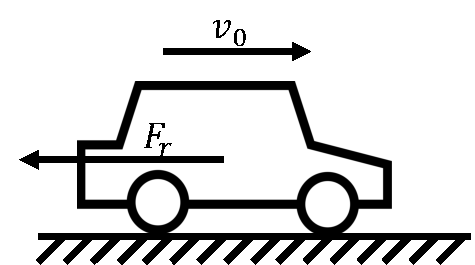
\includegraphics[width=.3\linewidth]{braking_diagram} 
    \end{center}
  \end{frame}
  
  \begin{frame}
    \frametitle{Common Modeling Choices with Non-parametric Regression}
    \begin{itemize}
    \item A straight-forward modeling choice to ignore the difference in conditions. The relation between the speed and distance can be modeled as
\begin{equation*}
y = f(x) + \epsilon,\quad f \sim GP, \label{eqn:simple_model}
\end{equation*}
    \item Alternatively, we can model each condition separately, i.e., $f_d \sim GP, d=1,\ldots,D$.
    \end{itemize}
    \begin{center}
    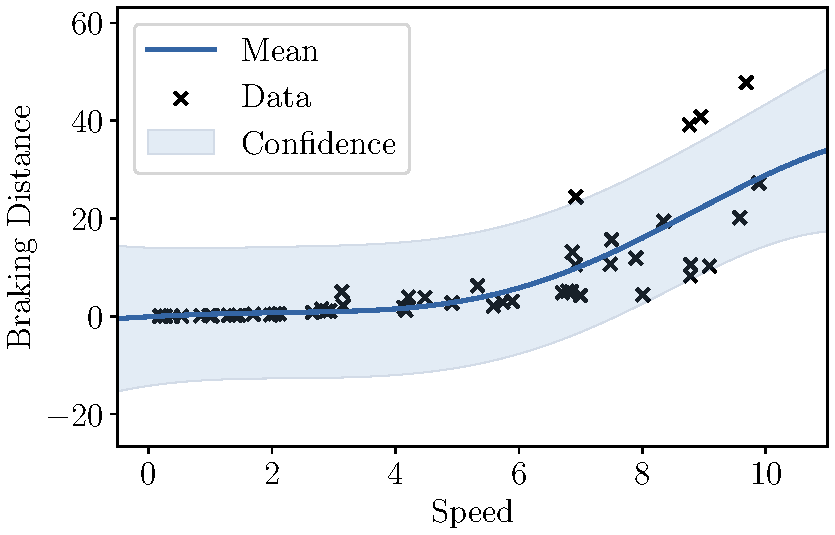
\includegraphics[width=.35\linewidth]{braking_all} ~ 
    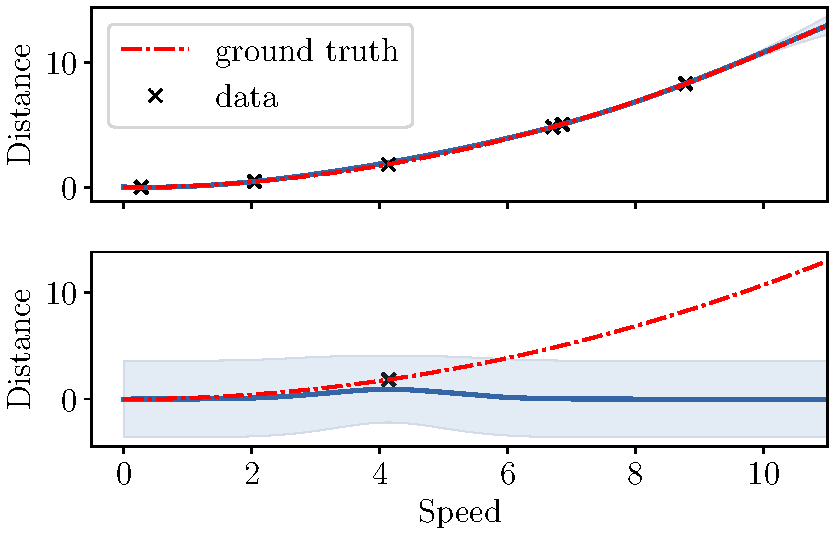
\includegraphics[width=.35\linewidth]{braking_separate}
    \end{center}
  \end{frame}

  \begin{frame}
    \frametitle{Modeling the Conditions Jointly}
    \begin{itemize}
    \item A probabilistic approach is to assume a latent variable.
    \item With a latent variable $\hV_d$, the relation between speed and distance for the condition $d$ is, then, modeled as
\begin{equation}
y = f(x, \hV_d) + \epsilon,\quad f \sim GP,\quad \hV_d \sim \mathcal{N}(0,\I). \label{eqn:model_latentinfo}
\end{equation}
    \item A special Bayesian GPLVM?
    \begin{itemize}
    \item  Efficiency, $O(N^3D^3)$ or $O(NDM^2)$. 
    \item The balance among different conditions in inference.
     \end{itemize}
    \end{itemize}
    \begin{center}
    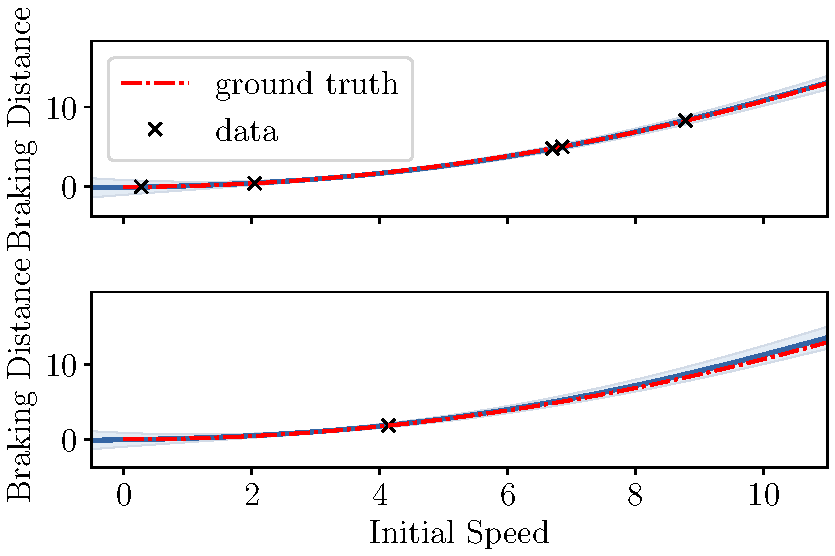
\includegraphics[width=.35\linewidth]{braking_lvmogp} ~ 
    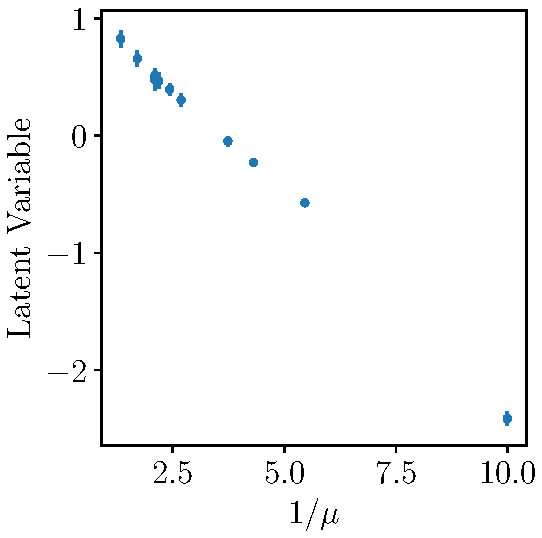
\includegraphics[width=.22\linewidth]{braking_latent_var}
    \end{center}
  \end{frame}

  \begin{frame}
    \frametitle{Latent Variable Multiple Output Gaussian Processes (LVMOGP)}
    \begin{itemize}
    \item We propose a new model which assumes the covariance matrix can be decomposed as a Kronecker product of the covariance matrix of the latent variables $\K^H$ and the covariance matrix of the inputs $\K^X$. 
    \item The probabilistic distributions of LVMOGP is defined as
\begin{equation}
p(\yM_: | \fM_:) = \gaussianDist{\yM_:}{\fM_:}{\sigma^2\I}, \quad p(\fM_:| \xM, \hM) = \gaussianDist{\fM_:}{0}{\K^H \otimes \K^X},  \label{eqn:lomogp}
\end{equation}
where the latent variables $\hM$ have unit Gaussian priors, $\hV_d \sim \mathcal{N}(0,\I)$
   \item This is a special case of the model in (\ref{eqn:model_latentinfo}).
  \end{itemize}
  \end{frame}

  \begin{frame}
    \frametitle{Scalable Variational Inference}
    \begin{itemize}
    \item Sparse GP approximation with $\uM \in \mathbb{R}^{M_X \times M_H}$:
    \begin{equation*}
\log p(\yM|\xM, \hM) \geq \expectationDist{\log p(\yM_:|\fM_:)}{q(\fM|\uM)q(\uM)} + 
\expectationDist{\log \frac{p(\fM|\uM, \xM, \hM)  p(\uM)}{q(\fM|\uM)q(\uM)}}{q(\fM|\uM)q(\uM)} 
\end{equation*}
   \item Lower bounding the marginal likelihood
   \begin{equation}
\log p(\yM|\xM) \geq  \mathcal{F} -\KL{q(\uM)}{p(\uM)} -\KL{q(\hM)}{p(\hM)},\label{eqn:lower_bound}
\end{equation}
  \end{itemize}
  \end{frame}
  
  \begin{frame}
    \frametitle{Closed-form Variational Lower Bound (SVI-GP)}
    \begin{itemize}
    \item It is known that the optimal posterior distribution of $q(\uM)$ is a Gaussian distribution \citep{Titsias2009, MatthewsEtAl2016}. With an explicit Gaussian definition of $q(\uM) = \gaussianDist{\uM}{\mM}{\sM^U}$, the integral in $\mathcal{F}$ has a closed-form solution:
\begin{align*}
\mathcal{F} = 
&-\frac{ND}{2}\log 2\pi \sigma^2 -\frac{1}{2\sigma^2} \yM_:^\top\yM_: -\frac{1}{2\sigma^2}\Tr\left(\K^{-1}_{uu} \Phi \K^{-1}_{uu} (\mM_{:}\mM_{:}^\top+\sM^{U}) \right)  \nonumber\\
&+\frac{1}{\sigma^2}\yM_:^\top \Psi \K^{-1}_{uu} \mM_{:}  -\frac{1}{2\sigma^2} \left( \psi -\tr{\K^{-1}_{uu} \Phi} \right) \label{eqn:F_3}
\end{align*}
where $\psi = \expectationDist{\tr{\K_{ff}}}{q(\hM)}$, $\Psi = \expectationDist{\K_{fu}}{q(\hM)}$ and $\Phi = \expectationDist{\K_{fu}^\top\K_{fu}}{q(\hM)}$
\item The computational complexity of the closed-form solution is $O(NDM_X^2M_H^2)$.
  \end{itemize}
  \end{frame}
  
    \begin{frame}
    \frametitle{More Efficient Formulation}
    \begin{itemize}
    \item The Kronecker product decomposition of covariance matrices are not exploited.
    \item Firstly, the expectation computation can be decomposed,
\begin{equation}
\psi =  \psi^H \tr{\K^X_{ff}}, \quad
\Psi = \Psi^H \otimes \K^X_{fu}, \quad
\Phi = \Phi^H \otimes \left((\K^X_{fu})^\top \K^X_{fu}) \right),
\end{equation}
where $\psi^H = \expectationDist{\tr{\K^H_{ff}}}{q(\hM)}$, $\Psi^H = \expectationDist{\K^H_{fu}}{q(\hM)}$ and $\Phi^H = \expectationDist{(\K^H_{fu})^\top\K^H_{fu}}{q(\hM)}$.
  \end{itemize}
  \end{frame}
  
      \begin{frame}
    \frametitle{More Efficient Formulation}
    \begin{itemize}
    \item Secondly, we assume a Kronecker product decomposition of the covariance matrix of $q(\uM)$, i.e., $\Sigma^U = \Sigma^H \otimes \Sigma^X$.
    \item The number of variational parameters in the covariance matrix from $M_X^2M_H^2$ to $M_X^2 + M_H^2$.
    \item The direct computation of Kronecker products is completely avoided.
   \begin{align*}
\mathcal{F}
=& -\frac{ND}{2}\log 2\pi \sigma^2 -\frac{1}{2\sigma^2} \yM_:^\top\yM_: \\
&-\frac{1}{2\sigma^2}\tr{ \mM^\top ((\K_{uu}^X)^{-1} \Phi^C (\K_{uu}^X)^{-1}) \mM (\K_{uu}^H)^{-1} \Phi^H (\K_{uu}^H)^{-1} }\nonumber \\
 &-\frac{1}{2\sigma^2}\tr{ (\K_{uu}^H)^{-1} \Phi^H (\K_{uu}^H)^{-1} \sM^{H} } \tr{ (\K_{uu}^X)^{-1} \Phi^X (\K_{uu}^X)^{-1} \sM^{X}} \nonumber \\
& \ldots
\end{align*}
  \end{itemize}
  \end{frame}
  
      \begin{frame}
    \frametitle{Prediction}
    \begin{itemize}
    \item Given both a set of new inputs $\xM^*$ with a set of new scenarios $\hM^*$, the prediction of noiseless observation $\fM^*$ can be computed in closed-form.
    \begin{align*}
q(\fM_{:}^* | \xM^*, \hM^*) =& \int p(\fM_{:}^* | \uM_{:},  \xM^*, \hM^*) q(\uM_{:}) \dif{\uM_{:}} \\
=& \gaussianDist{\fM_{:}^*}{\K_{f^* u}\K_{uu}^{-1}\mM_{:}}{\K_{f^*f^*}-\K_{f^*u}\K_{uu}^{-1}\K_{f^*u}^\top+\K_{f^* u}\K_{uu}^{-1}\sM^{U}\K_{uu}^{-1}\K_{f^* u}^\top},  
\end{align*}
    \item For a regression problem, we are often more interested in predicting for the existing condition from the training data. We can approximate the prediction by integrating the above prediction equation with $q(\hM)$,
\begin{align*}
q(\fM_{:}^* | \xM^*) = \int q(\fM_{:}^* | \xM^*, \hM) q(\hM) \dif{\hM}.
\end{align*}
  \end{itemize}
  \end{frame}

      \begin{frame}
    \frametitle{Missing Data}
    \begin{itemize}
    \item The model described previously assumes that for $N$ different inputs, we observe them in all the $D$ different conditions.
    \item In real world problems, we often collect data at a different set of inputs for each scenario, i.e., for each condition $d$, $d=1, \dots, D$.
    \item The proposed model can be extended to handle this case by reformulating the $\mathcal{F}$ as
\begin{align*}
\mathcal{F} = \sum_{d=1}^D
&-\frac{N_d}{2}\log 2\pi \sigma_d^2 -\frac{1}{2\sigma^2_d} \yM_d^\top\yM_d -\frac{1}{2\sigma^2_d}\Tr\left(\K^{-1}_{uu} \Phi_d \K^{-1}_{uu} (\mM_{:}\mM_{:}^\top+\sM^{U}) \right)  \nonumber\\
&+\frac{1}{\sigma^2_d}\yM_d^\top \Psi_d \K^{-1}_{uu} \mM_{:}  -\frac{1}{2\sigma^2_d} \left( \psi_d -\tr{\K^{-1}_{uu} \Phi_d} \right),
\end{align*}
where $\Phi_d = \Phi_d^H \otimes \left((\K^X_{f_du})^\top \K^X_{f_du}) \right)$, $\Psi_d = \Psi_d^H \otimes \K^X_{f_du}$, $\psi_d = \psi_d^H \otimes \tr{\K^X_{f_df_d}}$
  \end{itemize}
  \end{frame}

      \begin{frame}
    \frametitle{Related Works}
    \begin{itemize}
    \item Multiple Output Gaussian Processes /Multi-task Gaussian proccesses: \citet{Alvarez2012}  \citep{Goovaerts1997}  \citep{Bonilla2007}
    \item Our method reduces
computationally complexity to $O(\max(N,M_H)\max(D,M_X)\max(M_X,M_H))$ when there are no missing data.
\item An additional advantage of our method is that it can easily be parallelized using mini-batches like in \citep{HensmanEtAl2016}.
\item The idea of modeling latent information about different conditions jointly with the modeling of data points is related to the style and content model by \cite{TenenbaumFree2000}.
  \end{itemize}
  \end{frame}
  
      \begin{frame}
    \frametitle{Experiments on Synthetic Data}
    \begin{itemize}
    \item 100 different uniformly sampled input locations (50 for training and 50 for testing), where each corresponds to 40 different conditions. An observation noise with variance 0.3 is added onto the training data
    \item We compare LVMOGP with two other methods: GP with independent output dimensions (GP-ind) and LMC (with a full rank coregionalization matrix).
\item First dataset without missing data.

  \end{itemize}
      \begin{center}
          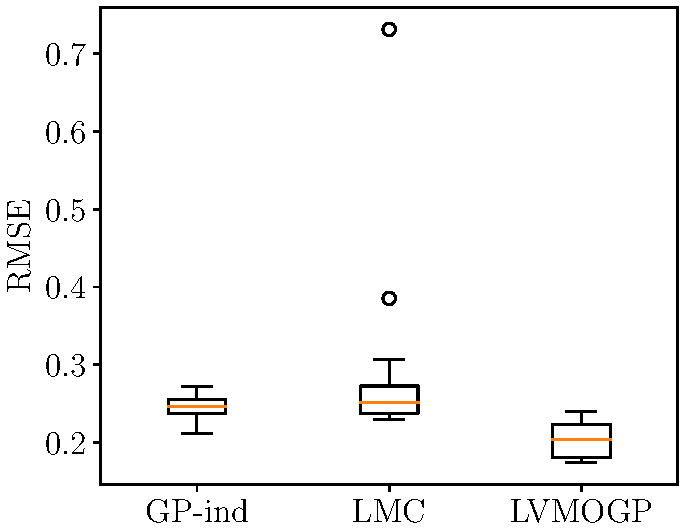
\includegraphics[width=.3\linewidth]{syn_results}
     \end{center}
  \end{frame}

      \begin{frame}
    \frametitle{Experiments on Synthetic Data with Missing Data}
    \begin{itemize}
    \item To generate a dataset with uneven numbers of training data in different conditions, we group the conditions into 10 groups. Within each group, the numbers of training data in four conditions are generated through a three-step stick breaking procedure with a uniform prior distribution (200 data points in total).
    \item We compare LVMOGP with two other methods: GP with independent output dimensions (GP-ind) and LMC (with a full rank coregionalization matrix).
    \item GP-ind: $0.43\pm0.06$, LMC:$0.47\pm0.09$, LVMOGP $0.30\pm0.04$
  \end{itemize}
      \begin{center}
        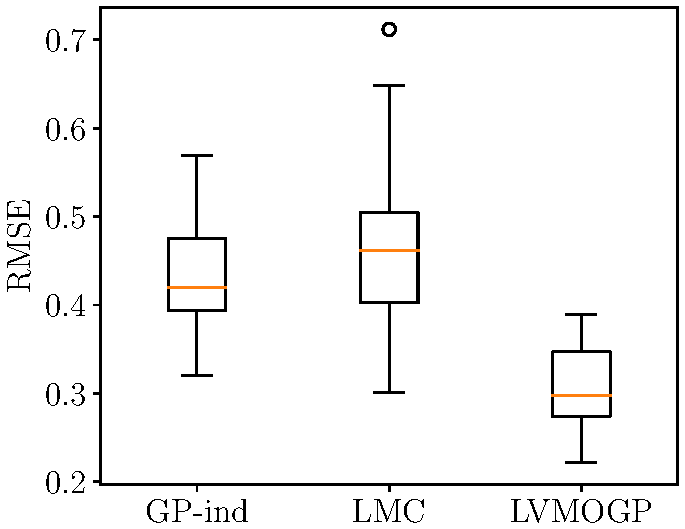
\includegraphics[width=.3\linewidth]{syn_md_results}
        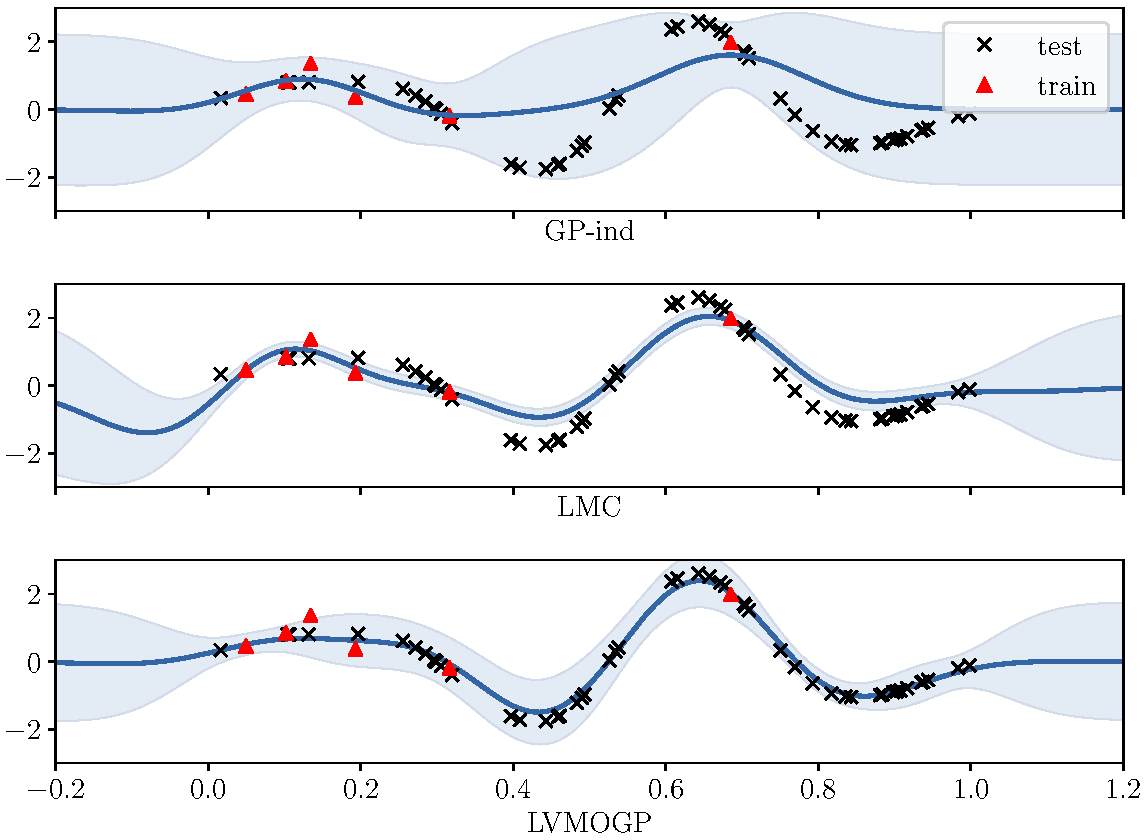
\includegraphics[width=.32\linewidth]{syn_md_example}
     \end{center}
  \end{frame}
  
       \begin{frame}
    \frametitle{Experiment on Servo Data}
    \begin{itemize}
    \item We apply our method to a servo modeling problem, in which the task to predict the rise time of a servomechanism in terms of two (continuous) gain settings and two (discrete) choices of mechanical linkages \citep{Quinlan1992}.
    \item The two choices of mechanical linkages: 5 types of motors and 5 types of lead screws.
    \item We take 70\% of the dataset as training data and the rest as test data, and randomly generated 20 partitions.
    \item GP-WO: $1.03\pm0.20$, GP-ind: $1.30\pm0.31$, GP-OH: $0.73\pm0.26$, LMC:$0.69\pm0.35$, LVMOGP $0.52\pm0.16$
  \end{itemize}
      \begin{center}
        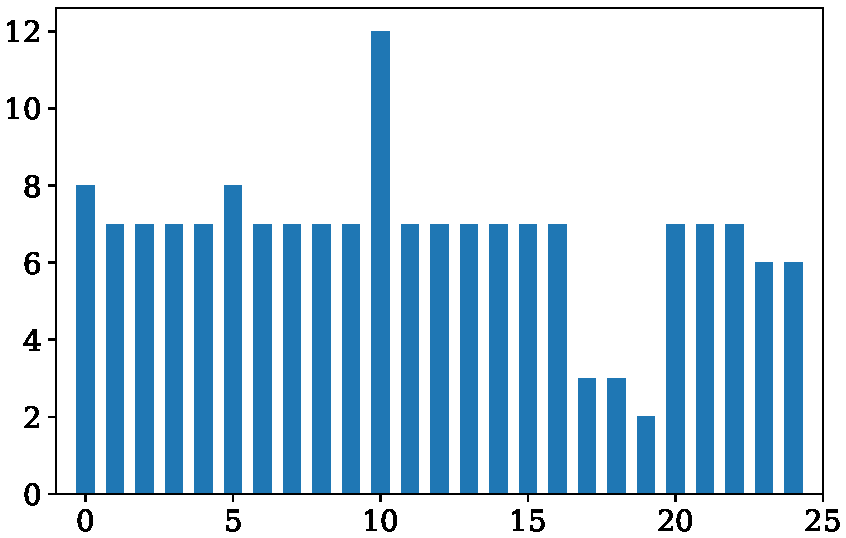
\includegraphics[width=.32\linewidth]{servo_data}~
        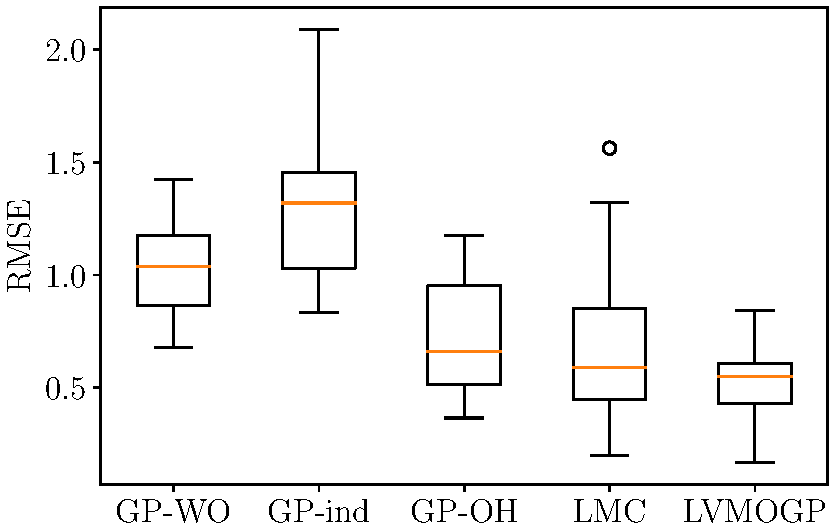
\includegraphics[width=.32\linewidth]{servo_results}~
        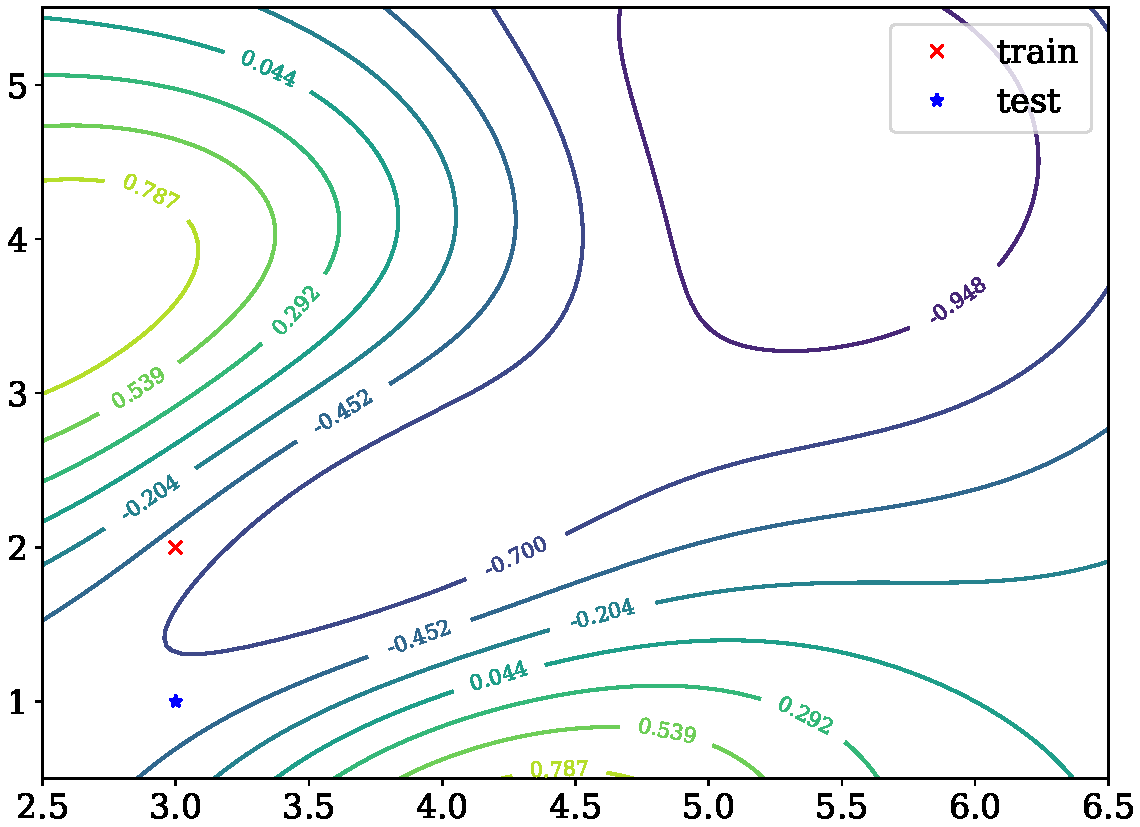
\includegraphics[width=.29\linewidth]{servo_levelset}
     \end{center}
  \end{frame}

       \begin{frame}
    \frametitle{Experiment on Sensor Imputation}
    \begin{itemize}
    \item We apply our method to impute multivariate time series data with massive missing data. We take a in-house multi-sensor recordings including a list of sensor measurements such as temperature, carbon dioxide, humidity, etc. \citep{ZamoraEtAl2014}.
    \item The measurements are recorded every minutes for roughly a month and smoothed with 15 minute means.
    \item We mimic the scenario of massive missing data by randomly taking out 95\% of the data entries and aim at imputing all the missing values.
    \item GP-ind: $0.85\pm0.09$, LMC:$0.59\pm0.21$, LVMOGP $0.45\pm0.02$
  \end{itemize}
      \begin{center}
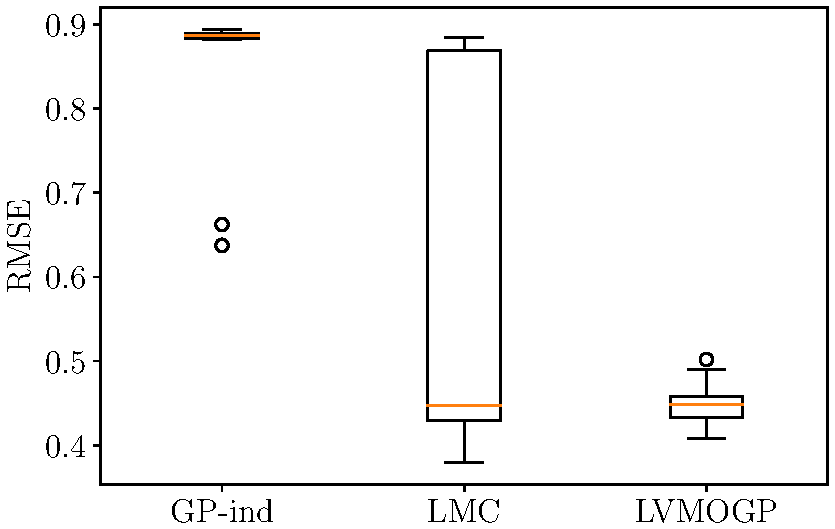
\includegraphics[width=.3\linewidth]{sml2010_results}
     \end{center}
  \end{frame}

       \begin{frame}
    \frametitle{Conclusion}
    \begin{itemize}
    \item The common practices such as one-hot encoding cannot efficiently model the relation among different conditions and are not able to generalize to a new condition at test time. 
    \item We propose to solve this problem in a principled way, where we learn the latent information of conditions into a latent space as part of the regression model. 
    \item By exploiting the Kronecker product decomposition in the variational posterior, our inference method are able to achieve the same computational complexity as sparse GP with independent observations. 
    \item As shown repeatedly in the experiments, the Bayesian inference of the latent variables in LVMOGP avoids the overfitting problem in LMC.  \end{itemize}
  \end{frame}
 
 \begin{frame}
  \frametitle{Reference}
  \footnotesize
\bibliographystyle{plainnat}
\bibliography{./multi_out}
\end{frame}

\end{document}

